% Appendix A

\chapter{Data Samples} % Main appendix title

\label{Appendix A} % For referencing this appendix elsewhere, use \ref{AppendixA}
Initial dataset looked like Figure \ref{fig:Initial BIIS  Data}. After processing ans eliminating redundancy the data set looks like \ref{fig:Processed BIIS Data}.\\
Credit column is added as there was no valid credit column in the given data set. Credit was calculated from the obtained total marks and grade.\\Similarly Cgpa column was also created as there was no valid cgpa column in majority of the given data sets.

\begin{figure}[H]
   \centering
  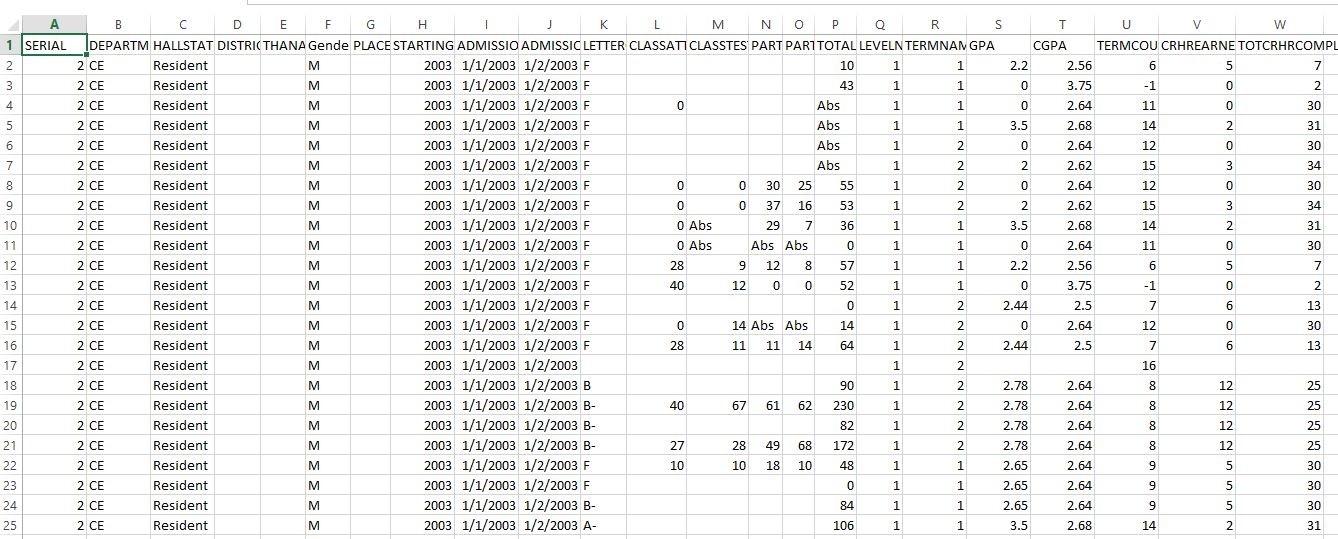
\includegraphics[width=\linewidth]{Figures/data.jpg}
  \decoRule
  \caption[BIIS Data]{BIIS Data}
  \label{fig:Initial BIIS  Data}
\end{figure}

\begin{figure}[H]
   \centering
  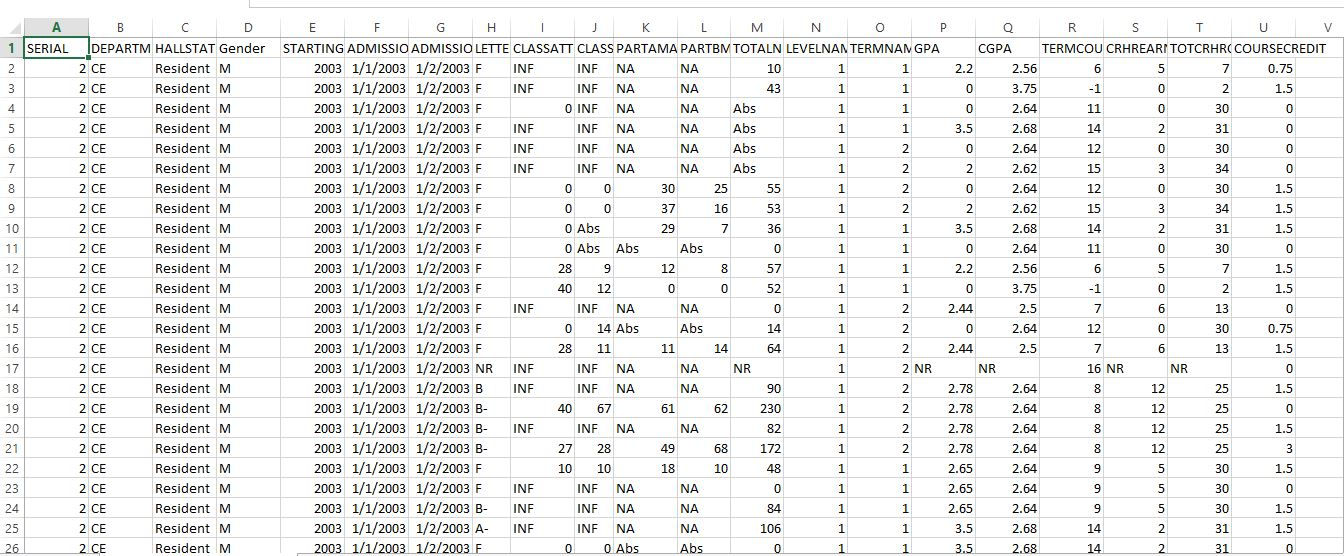
\includegraphics[width=\linewidth]{Figures/data1.jpg}
  \decoRule
  \caption[Processed BIIS Data]{Processed BIIS Data}
  \label{fig:Processed BIIS  Data}
\end{figure}